\documentclass[12pt,letterpaper]{article}
\usepackage[margin=.7in,headheight=18pt,headsep=17pt,footskip=28pt]{geometry}
\usepackage{tikz,fancyhdr,amssymb}
\usetikzlibrary{arrows.meta}
\pdfmapfile{+cm.map}\pdfmapfile{+cmextra.map}\pdfmapfile{+symbols.map}\pdfmapfile{+latxfont.map}
\renewcommand{\familydefault}{\sfdefault}
\setlength{\parindent}{0pt}\setlength{\parskip}{9pt}
\pagestyle{fancy}\fancyhf{}
\fancyhead[L]{\small Week 67 / Meeting on shortest roads / Grades 3--5}
\fancyfoot[L]{\footnotesize Bellingham Math Circle / Week 67 / GGT67-S-v1}
\fancyfoot[R]{\footnotesize\thepage}\renewcommand{\headrulewidth}{.4pt}

\newcommand{\problem}[2]{\par\textbf{Problem #1:} #2\par}
\newcommand{\grid}[1]{\draw[gray!65,line width=.6pt,step=1] (0,0) grid (#1,#1);\foreach \x in {0,...,#1}\foreach \y in {0,...,#1}\fill (\x,\y) circle (1.7pt);}
\newcommand{\home}[3]{\node[draw,circle,fill=white,inner sep=3pt,font=\bfseries] at (#1,#2){#3};}
\newcommand{\cube}{
\coordinate (000) at (0,0);\coordinate (100) at (3,0);\coordinate (110) at (3,3);\coordinate (010) at (0,3);
\coordinate (001) at (1.2,1.1);\coordinate (101) at (4.2,1.1);\coordinate (111) at (4.2,4.1);\coordinate (011) at (1.2,4.1);
\draw[line width=1pt] (000)--(100)--(110)--(010)--cycle (001)--(101)--(111)--(011)--cycle (000)--(001) (100)--(101) (110)--(111) (010)--(011);
\foreach \s in {000,100,110,010,001,101,111,011}{\node[fill=white,circle,draw,inner sep=2pt,font=\small] at (\s){\s};}}
\begin{document}
Travel along roads from dot to dot. Each road counts as one step. A shortest route uses the fewest steps. Routes may share roads; draw their colors side by side.

A meeting dot works when \textbf{each pair of homes has a shortest route through it}. The meeting dot may also be a home. Keep all three homes and the meeting dot fixed while checking the three pairs. One partner draws the routes in three colors; the other checks them.

\begin{center}
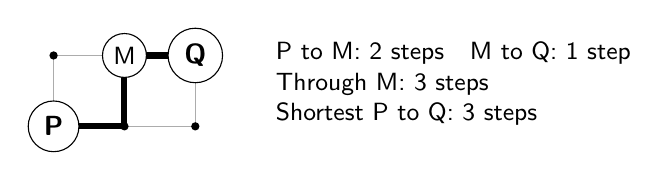
\begin{tikzpicture}[x=.9cm,y=.9cm,font=\small]
\draw[gray!65,step=1] (0,0) grid (2,1);\foreach \x in {0,1,2}\foreach \y in {0,1}\fill (\x,\y) circle (1.5pt);
\draw[line width=2.2pt] (0,0)--(1,0)--(1,1)--(2,1);
\home{0}{0}{P}\home{2}{1}{Q}\node[draw,circle,fill=white,inner sep=2pt] at (1,1){M};
\node[align=left,anchor=west] at (3,.6){P to M: 2 steps\quad M to Q: 1 step\\Through M: 3 steps\\Shortest P to Q: 3 steps};
\end{tikzpicture}
\end{center}
\problem{1}{Place a meeting counter so that it works for A, B, and C. Draw the three shortest routes through your meeting dot. Find every meeting dot that works on each board.}
\vspace{.25in}
\begin{center}
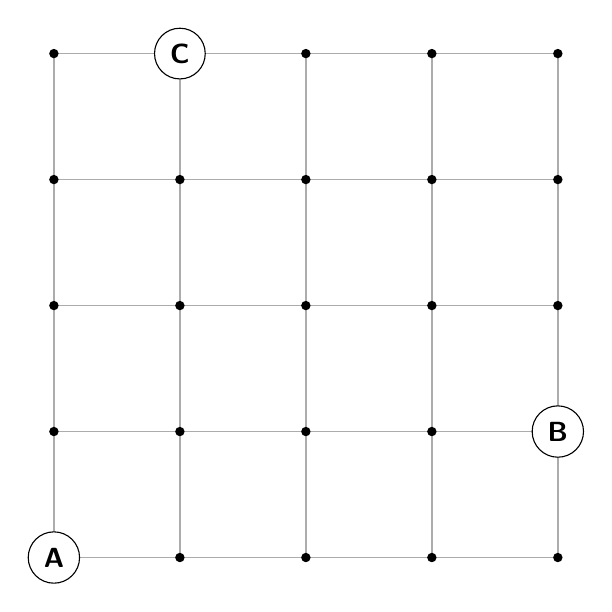
\begin{tikzpicture}[x=1.6cm,y=1.6cm]\grid{4}\home{0}{0}{A}\home{4}{1}{B}\home{1}{4}{C}\end{tikzpicture}\hfill
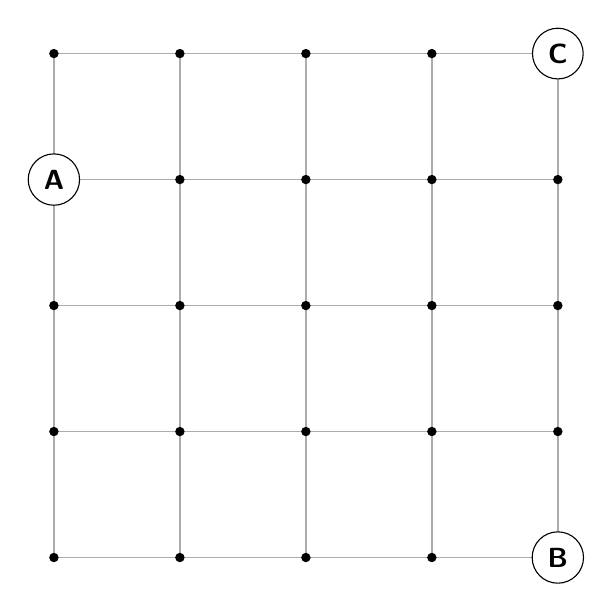
\begin{tikzpicture}[x=1.6cm,y=1.6cm]\grid{4}\home{0}{3}{A}\home{4}{0}{B}\home{4}{4}{C}\end{tikzpicture}
\end{center}
\vfill
\newpage
\problem{2}{Put A, B, and C at three different dots. Challenge your partner to find every meeting dot that works, then swap jobs. Can you place the homes so that no meeting dot works? Can you make more than one work? Keep a drawing of your attempts.}
\vspace{.25in}
\begin{center}
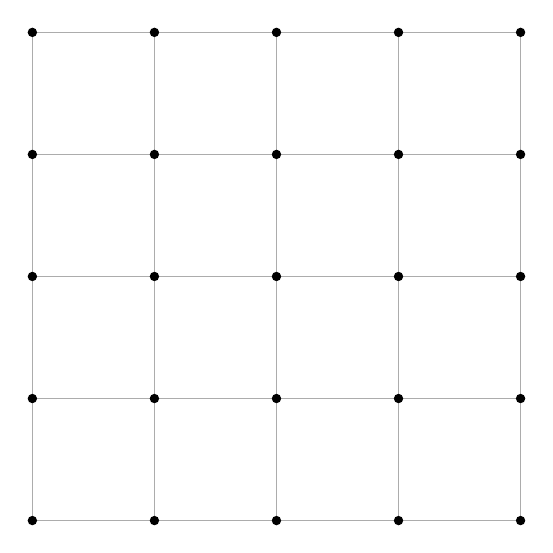
\begin{tikzpicture}[x=1.55cm,y=1.55cm]\grid{4}\end{tikzpicture}\hfill
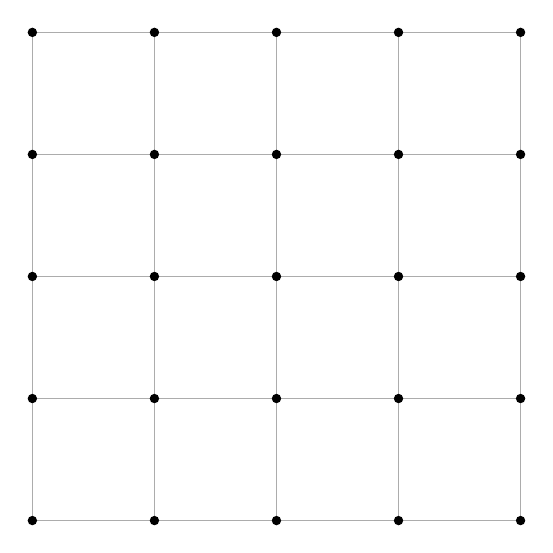
\begin{tikzpicture}[x=1.55cm,y=1.55cm]\grid{4}\end{tikzpicture}
\vspace{.6in}

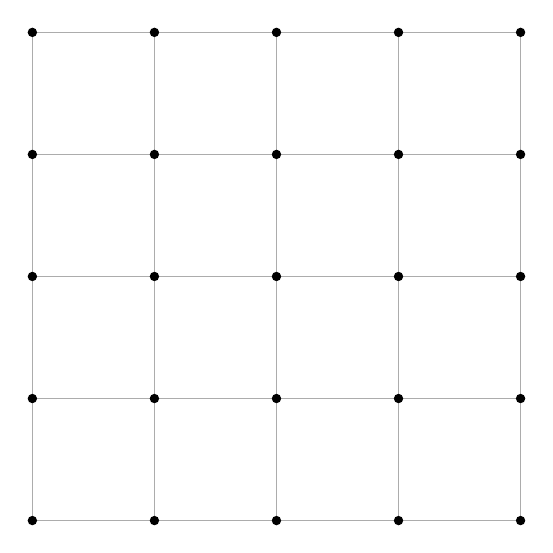
\begin{tikzpicture}[x=1.55cm,y=1.55cm]\grid{4}\end{tikzpicture}\hfill
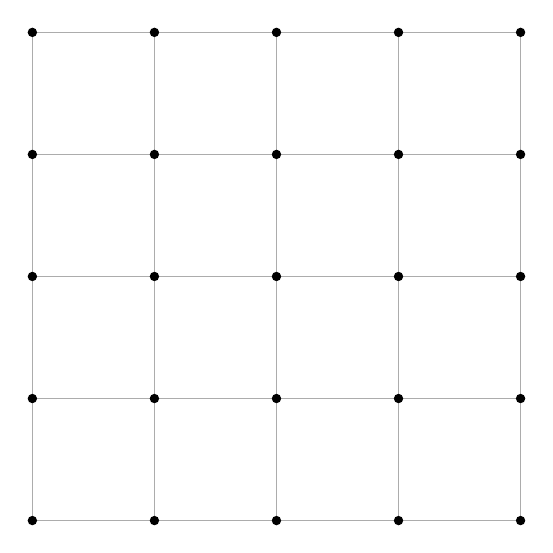
\begin{tikzpicture}[x=1.55cm,y=1.55cm]\grid{4}\end{tikzpicture}
\end{center}
\newpage
\problem{3}{Find every meeting dot that works for A, B, and C on each map. If none works, explain why every possible dot fails. Each line between neighboring dots is one road, even when drawn longer.}
\begin{center}
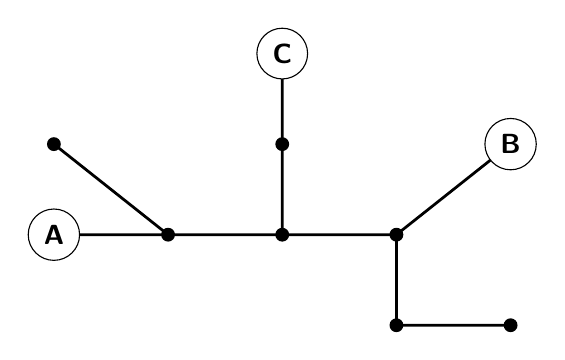
\begin{tikzpicture}[x=1.45cm,y=1.15cm]
\foreach \n/\x/\y in {a/0/0,u/1/0,v/2/0,w/3/0,b/4/1,c/2/2,t/2/1,s/3/-1,r/4/-1,q/0/1}{\coordinate (\n) at (\x,\y);}
\draw[line width=1pt] (a)--(u)--(v)--(w)--(b) (v)--(t)--(c) (w)--(s)--(r) (u)--(q);
\foreach \n in {a,u,v,w,b,c,t,s,r,q}\fill (\n) circle (2.5pt);
\home{0}{0}{A}\home{4}{1}{B}\home{2}{2}{C}
\end{tikzpicture}
\end{center}
\vspace{.2in}
\begin{center}
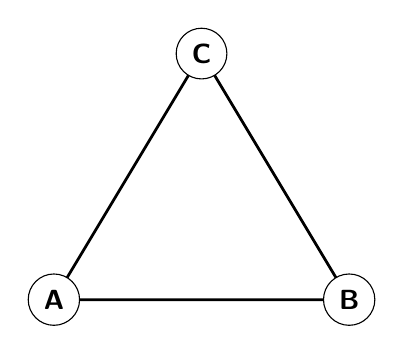
\begin{tikzpicture}[x=1.25cm,y=1.25cm]
\draw[line width=1pt] (0,0)--(3,0)--(1.5,2.5)--cycle;
\home{0}{0}{A}\home{3}{0}{B}\home{1.5}{2.5}{C}
\end{tikzpicture}\hspace{1.0in}
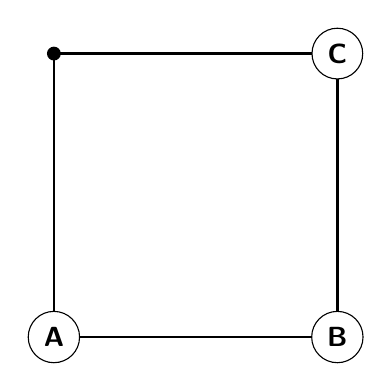
\begin{tikzpicture}[x=1.2cm,y=1.2cm]
\draw[line width=1pt] (0,0)--(3,0)--(3,3)--(0,3)--cycle;
\fill (0,3) circle (2.5pt);\home{0}{0}{A}\home{3}{0}{B}\home{3}{3}{C}
\end{tikzpicture}
\end{center}
\vspace{.35in}\rule{\linewidth}{.4pt}\par\vspace{.35in}\rule{\linewidth}{.4pt}\par\vspace{.35in}\rule{\linewidth}{.4pt}
\newpage
Each dot on these maps has a three-digit label. A road changes exactly one digit. Crossed roads connect only at a labeled dot.
\begin{center}
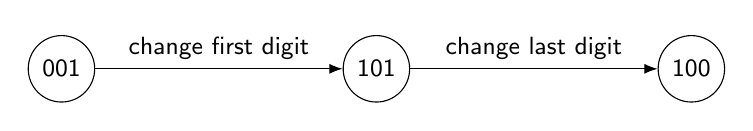
\begin{tikzpicture}[font=\small]
\node[draw,circle] (a) at (0,0){001};\node[draw,circle] (b) at (4,0){101};\node[draw,circle] (c) at (8,0){100};
\draw[-{Latex}] (a)--node[above]{change first digit}(b);
\draw[-{Latex}] (b)--node[above]{change last digit}(c);
\end{tikzpicture}
\end{center}
\problem{4}{The homes are 000, 110, and 101 on the left map, and 001, 010, and 111 on the right. Mark the homes. Find every meeting dot that works and draw the three shortest routes through it.}
\vspace{.15in}
\begin{center}
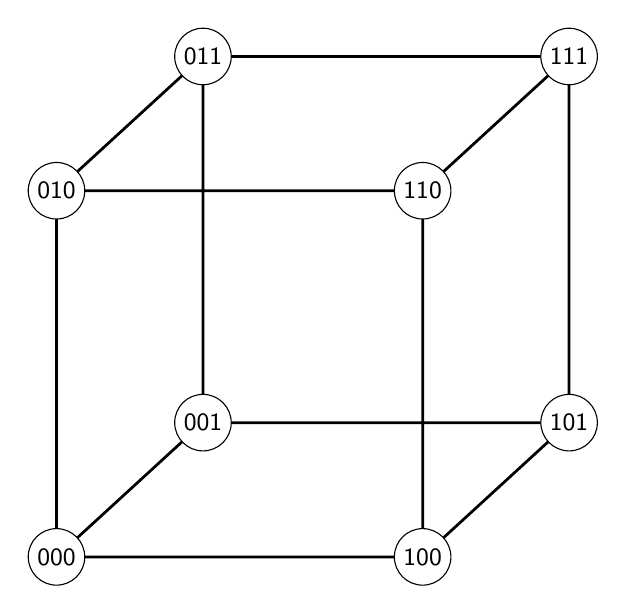
\begin{tikzpicture}[x=1.55cm,y=1.55cm]\cube\end{tikzpicture}\hfill
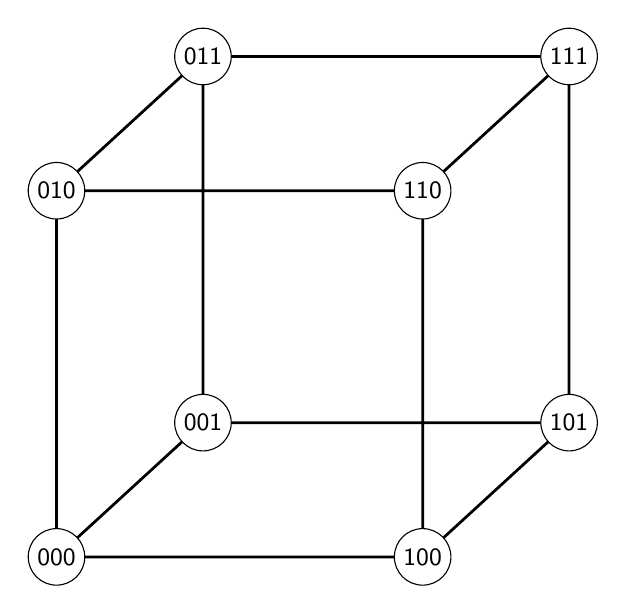
\begin{tikzpicture}[x=1.55cm,y=1.55cm]\cube\end{tikzpicture}
\end{center}
\vspace{.2in}
\problem{5}{Choose three new homes on a cube map. Can you predict the meeting label from the home labels? Explain a rule that works for every choice of three homes.}
\vspace{.35in}\rule{\linewidth}{.4pt}\par\vspace{.4in}\rule{\linewidth}{.4pt}\par\vspace{.4in}\rule{\linewidth}{.4pt}
\end{document}
